\documentclass[A4paper, 12pt, oneside]{book}
\usepackage[left=1in, right=1in]{geometry}
\usepackage[czech]{babel}
\usepackage{inputenc}
\usepackage[T1]{fontenc}
\usepackage{graphicx, enumitem}
\usepackage{epstopdf}
\usepackage{setspace}
\usepackage{csquotes}
\usepackage{amsmath, amssymb, amsthm}
\usepackage[inline]{asymptote}
\usepackage{esdiff, icomma, subcaption}
\usepackage{blindtext}

\usepackage[backend=biber, url=true, sorting=none]{biblatex}
\usepackage{url}
\addbibresource{soc.bib}

\newcommand{\B}[1]{\textbf{#1}}
\renewcommand{\S}[1]{\textsc{#1}}
\newcommand{\I}[1]{\textit{#1}}
\newcommand{\mB}[1]{\mathbf{#1}}
\newcommand{\ap}{{\,\prime}}
\newcommand{\abs}[1]{\lvert #1 \,\rvert}

\setstretch{1.3}
\renewcommand*\contentsname{Obsah}
\renewcommand{\theequation}{\arabic{equation}}

\begin{document}
\voffset = -10mm
\begin{center}
	{\LARGE \B{\S{Středoškolská odborná činnost}}} \\
	{\large \B{{Obor č. 2: Fyzika}}}
	\vfill
	{\Huge \B{Mechanika rodin planetek \\ s aplikací na rodinu Eunomia}}
\end{center}
	\vfill
{\large \bfseries Adam Křivka \\
	Jihomoravský kraj \hfill Brno 2018}

\newpage

TODO: Ostatní nutné úvodní stránky pro SOČku \ldots

\newpage
\tableofcontents
\newpage
%\addcontentsline{toc}{section}{Úvod}

\chapter{Úvod do nebeské mechaniky}
TODO: Úvod
\vspace{40mm}
\section{Pohybové rovnice}
Pohybová rovnice je matematicky zapsaný fyzikální vztah, který popisuje možné pohyby těles v daném prostředí \cite{wiki:eqm}. Řešením pohybové rovnice je funkce, popisující polohu a rychlost každého zkoumaného tělesa v závislosti na čase. Přitom potřebujeme znát počáteční podmínky --- polohy a rychlosti těles na začátku. Pohybová rovnice bývá ve tvaru diferenciální rovnice, což je rovnice, která vyjadřuje vztah mezi nějakou funkcí a jejími derivacemi, což je okamžitá změna hodnoty funkce při velmi malé změně argumentu, v našem případě času. 

V následující části se pokusíme nalézt řešení pohybové rovnice pro tělesa ve sluneční soustavě. Zákony, jimiž se budou naše tělesa řídit, jsou Newtonův gravitační zákon a Newtonovy pohybové zákony, které byly poprvé definovány již v roce 1687.
\subsection{Rovnice pro dvě tělesa} \label{sec:2body}
Omezme se nyní na dvě tělesa a nalezněme řešení tzv.\ problému dvou těles, někdy také Keplerovy úlohy. To znamená, že se pokusíme odvodit funkci, popisující polohu a rychlost obou těles v závisloti na čase. 

Nacházíme se v inerciální vztažné soustavě, což je taková vztažná soustava, kde platí první Newtonův zákon. Jako bod v klidu si zvolme těžiště soustavy. Pro síly působící na obě tělesa podle Newtonova gravitačního zákona a druhého a třetího pohybového zákona platí
\begin{align} 
	\vec{F}_1 &= +G\frac{m_1m_2}{\abs{\vec{r}}^3}\vec{r} = m_1\vec{a}_1 \label{eq:newton1} \\
	\vec{F}_2 &= -G\frac{m_1m_2}{\abs{\vec{r}}^3}\vec{r} = m_2\vec{a}_2, \label{eq:newton2}
\end{align}
kde $G$ označuje gravitační konstantu, $m_1$, $m_2$ hmotnosti zkoumaných těles, $\vec{a}_1$, $\vec{a}_2$ vektory zrychlení těles (tj.\ druhé derivace polohových vektorů $\vec{r}_1$, $\vec{r}_2$ podle času) a $\vec{r}$ vektor udávající vzájemnou polohu těles, definovanou jako $\vec{r} = \vec{r}_2 - \vec{r}_1$. Součtem obou rovnic dostáváme
\begin{equation} \label{eq:mr0}
	\vec{F}_1 + \vec{F}_2 = m_1\vec{a_1} + m_2\vec{a_2} = 0.
\end{equation}
Vektor popisující polohu těžiště soustavy je $\vec{R} \equiv \frac{m_1\vec{r}_1 + m_2\vec{r}_2}{m_1 + m_2}$. Jeho druhou derivací podle času dostáváme zrychlení
\begin{equation*}
	\diff[2]{\vec{R}}{t} = \frac{m_1\vec{a_1} + m_2\vec{a_2}}{m_1+m_2} = 0,
\end{equation*}
které se podle \eqref{eq:mr0} rovná nule, takže se těžiště soustavy pohybuje konstantní rychlostí.
\newpage
Nyní se však přesuňme do soustavy neinerciální, kde je první z těles (běžně to hmotnější) nehybné. Řekněme, že nehybné těleso má index $1$, tedy nově $\vec{r}^\ap_1=0$, $\vec{r}^\ap_2=\vec{r}$ (tedy i $\vec{a}^\ap_2 = \vec{a}$) a $\vec{r}^\ap=\vec{r}$. Provedli jsme tedy v podstatě transformaci, kdy jsme ke každému vektoru přičetli $\vec{r}_1$.  Rovnici \eqref{eq:newton1} můžeme přepsat jako
\begin{align}
	\nonumber {\vec{a}} = Gm_2\frac{\vec{r}}{\abs{\vec{r}}^3} \\
		\diff[2]{\vec{r}}{t} - Gm_2\frac{\vec{r}}{\abs{\vec{r}}^3} = 0	
\end{align}
Často ještě definujeme gravitační paramter soustavy $\mu=Gm_2$.

I přesto, že tato diferenciální rovnice ještě není ve své konečné podobě vhodné k tomu, abychom z ní vyvodili následující vztah, prozradíme, že je jím funkce v polárních souřadnicích, popisující vzdálenost těles $r\equiv\abs{\vec{r}}$ v závisloti na úhlu $\theta$, který svírá přímka procházející oběma tělesy a nějaká zvolená referenční přímka. 
\begin{equation} \label{eq:polar}
	r(\theta)=\frac{p}{1+e\cos{(\theta-\omega)}}
\end{equation}
Pro naše účely se omezme na případ elipsy, kdy se v jednom z jejích ohnisek nachází centrální těleso.
$p$ označuje parametr elipsy, jehož velikost je určena hodnotou $\mu$ a pro který platí vztah
\begin{align}
	p=\frac{b^2}{a},
\end{align}
kde $a$ označuje délku hlavní poloosy, což je úsečka spojující střed elipsy s jedním z průsečíků elipsy s hlavní osou --- přímkou spojující ohniska, a $b$ označuje délku vedlejší poloosy, což je úsečka spojující střed elipsy s průsečíkem elipsy s přímkou kolmou na hlavní poloosu a procházející středem elipsy --- vedlejší osou (viz~\ref{fig:elip}).
Dále $e$, resp.\ $\omega$ jsou integrační konstanty a nazývají se excentricita, resp.\ argument pericentra. Pro excentricitu platí vztah
\begin{figure} 
	\centering
	\begin{asy}
		size(8cm,8cm);

		marker mark1 = marker(scale(circlescale*2)*unitcircle, Fill);

		real a = 1.5;
		real b = 1;

		draw(ellipse((0,0), a, b));

		draw((-1.5*a,0)--(1.5*a,0));
		draw((0,-b)--(0,b));
		draw((0,0), mark1);

		draw((a,0), mark1);
		draw((-a,0), mark1);
		label("$P$", (a,0), SE);
		label("$A$", (-a,0), SW);

		real F = sqrt((a-b)*(a+b));
		draw((F,0), mark1);
		draw((-F,0), mark1);
		label("$F_1$", (F,0), S);
		label("$F_2$", (-F,0), S);

		draw(brace((0,0), (a,0)));
		label("$a$", (a/2,0.25), N);

		draw(brace((0,0), (0,b)));
		label("$b$", (-0.25, b/2), W);

		draw((0,0)--(1.3,-1.1), arrow=EndArrow);
		draw(arc((0,0), 0.5, -degrees(atan(1.1/1.3)), 0));
		label("$\omega$", (0.35,-0.25), N);
	\end{asy}
	\caption{Eliptická oběžná dráha vesmírného tělesa. $a$ označuje délku hlavní poloosy, $b$ délku vedlejší poloosy, $F_1$ a $F_2$ označují polohy ohnisek elipsy, přičemž centrální těleso se nachází v bodě $F_1$, a $P$, resp.\ $A$ označují pericentrum, resp.\ apocentrum oběžné dráhy, tedy bod nejnižší, resp.\ nejvyšší vzdálenosti od centrálního tělesa, $\omega$ označuje argument pericentra.} \label{fig:elip}
\end{figure}
\begin{align}
	e=\sqrt{1-\frac{a^2}{b^2}},
\end{align}
a volně řečeno udává, jak moc se elipsa liší od kružnice.
Argument pericentra je úhel, který svírá hlavní osa s referenční přímkou. Platí pro něj vztah
\begin{align}
	\theta=\omega+f,
\end{align}
kde $f$ označuje pravou anomálii, což je úhel, který svírá hlavní osa s průvodičem tělesa.

\begin{figure} 
	\centering
	May-DO: Předělat do jednotného stylu obrázků.
	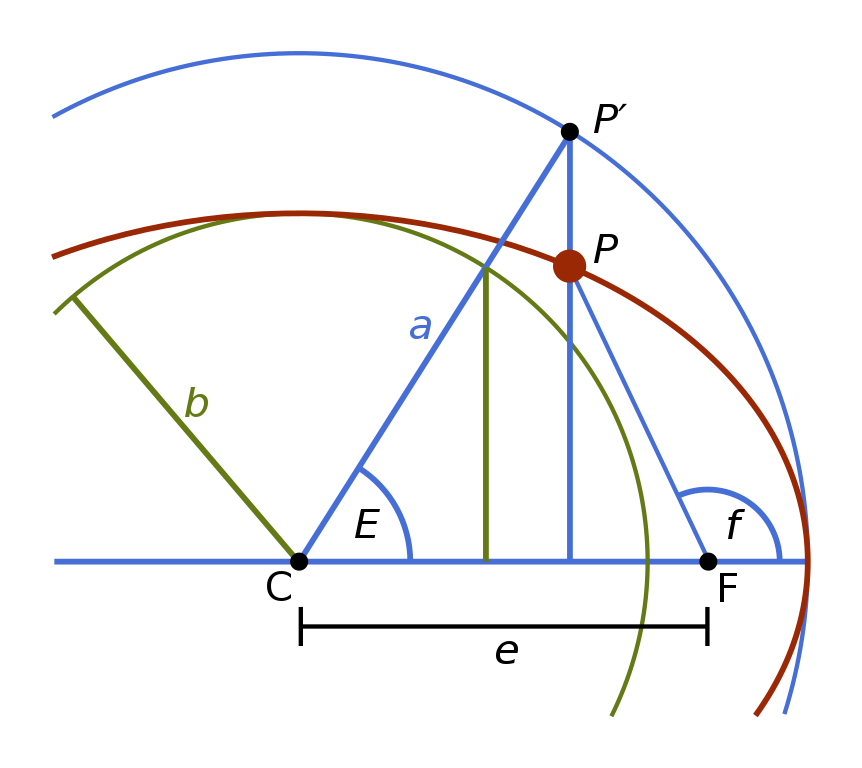
\includegraphics[width=0.5\textwidth]{obr/Eanomaly.png}
	\caption{Ilustrace vztahu mezi excentrickou anomálií $E$ a pravou anomálií $f$. $a$, resp. $b$ značí délku hlavní, resp. vedlejší poloosy, $P$ značí polohu tělesa na elipse, $C$ značí střed elipsy, $F$ značí ohnisko, ve kterém se nachází centrální těleso a $e$ značí excentricitu (vymazat??)} \label{fig:E}
\end{figure}

Uvědomme si, že jsme neodvodili závislost polohy tělesa na čase. Tuto závislost určuje Keplerova rovnice:
\begin{equation} \label{eq:kepler}
M = E + e\sin E
\end{equation}
kde $M$ označuje střední anomálii, $E$ excentrickou anomálii a $e$ excentricitu elipsy (viz obrázek~\ref{fig:E}). Mezi $E$ a pravou anomálií $f$ platí vztah
\begin{align} \label {eq:fE}
	\tan \frac{f}{2} = \sqrt{\frac{1+e}{1-e}\tan \frac{E}{2}}.
\end{align}

Anomálie mají úhlové jednotky, úhel $M$ ale nemůžeme zkonstruovat, nicméně je významný tím, že je lineárně závislý na čase. Je určen vztahem 
\begin{align} \label{eq:M}
	M=nt,
\end{align}
kde $n$ označuje střední denní pohyb, jinak řečeno průměrnou úhlovou rychlost. Pokud známe $E$, můžeme pomocí Keplerovy rovnice snadno spočítat $M$. Problém spočívá v tom, že nemůžeme vyjádřit $E$ v závisloti na $M$ konečným výrazem, ale pouze nekonečnou řadou nebo jej můžeme aproximovat iteračními nebo numerickými metodami.

\subsection{Rovnice pro N těles}
Jak vidíme, už i pro dvě tělesa se musíme k získání polohy tělesa v čase uchýlit k numerickým metodám. Ukazuje se, že obecný problém $N$ těles je analyticky neřešitelný\footnote{existují ale nějaká zajímavá speciální řešení, viz \cite{cohan12}.} a jediné aplikovatelné metody jsou metody přibližné analytické nebo numerické.

Uvažujme nyní $N$ těles --- respektive hmotných bodů, které na sebe vzájemně gravitačně působí v souladu s Newtonovým gravitačním zákonem. Pro libovolné těleso, označené indexem $j\in\{1,\,2,\,\dots,\,N\}$, je celková síla $F_j$, která na něj působí, výslednicí všech gravitačních sil způsobených ostatními tělesy, jak ukazuje následující rovnice.
\begin{align} 
	\vec{F}_j = m_j\vec{a}_j &= \sum_{\substack{i=1 \\ i\neq j}}^N G\frac{m_im_j}{\abs{\vec{r}_i-\vec{r}_j}^3}(\vec{r_i}-\vec{r_j}) \label{eq:nbody1}\\
		\vec{a}_j &= \sum_{\substack{i=1 \\ i\neq j}}^N \frac{Gm_i}{\abs{\vec{r}_i-\vec{r}_j}^3}(\vec{r_i}-\vec{r_j}) \label{eq:nbody2}
\end{align}
kde $\vec{r}_i-\vec{r}_j$ označuje vektor určující vzájemnou polohu těles $i$ a $j$, konkrétně jde o vektor s počátkem v tělese $j$ a vrcholem v tělese $i$; ostatní veličiny jsou definované analogicky jako v předchozí části.
\subsubsection{Eulerova metoda}
I přesto, že se následující integrační metoda v přesných numerických výpočtech zřídka používá, uvádíme ji zde z didaktických důvodů, neboť názorně ilustruje použití numerických metod pro řešení problému $N$ těles. Jak název napovídá, poprvé s ní v 18. století přišel švýcarský matematik Leonhard Euler.

Princip algoritmu spočívá v tom, že v libovolném čase můžeme z \eqref{eq:nbody2} vypočítat zrychlení každého tělesa. Pak, po zvolení určitého časového kroku, odpovídajícím způsobem změníme vektor rychlosti. Následně necháme všechna tělesa po dobu časového kroku pohybovat se po přímce konstantní rychlostí. Existují dvě verze Eulerovy metody, dopředná a zpětná, které se liší volbou rychlosti, se kterou necháváme pohybovat se po přímce, viz následující přesný popis obou metod a obrázek~\ref{fig:euler}.

Mějme zmiňovaných $N$ hmotných bodů, pro které platí \eqref{eq:nbody2}. Zaměřme se na jeden z nich a označme jeho počáteční polohu $\vec{r}(t_0)$ a počáteční rychlost $\vec{v}(t_0)$. K použití Eulerovy metody potřebujeme znát i počáteční polohy a rychlosti všech ostatních těles v systému. Dále vhodně zvolme velikost časového kroku $h$. V následujícíh třech krocích si ukážeme jednu iteraci algoritmu jak pro dopřednou, tak pro zpětnou metodu.

\begin{enumerate}
	\item Nechť je v čase $t_k$ poloha zvoleného bodu $\vec{r}(t_k)$ a rychlost $\vec{v}(t_k)$. Z \eqref{eq:nbody2} vypočítáme zrychlení $\vec{a}(t_k)$. 
	\item Položme $t_{k+1} = t_{k}+h$ a vypočítejme $\vec{v}(t_{k+1}) = \vec{v}(t_k) + h\cdot\vec{a}(t_k)$.\footnote{Můžeme porovnat se vzorcem pro rovnoměrný přímočarý pohyb, dobře známým ze středoškolského učiva: $v = v_0 + at$, podobně v kroku $3$ $s = s_0 + vt$}
	\item Pro dopřednou metodu vypočítejme $\vec{r}(t_{k+1})$ jako $\vec{r}(t_{k+1}) = \vec{r}(t_k) + h\cdot\vec{v}(t_k)$ a pro zpětnou jako $\vec{r}(t_{k+1}) = \vec{r}(t_k) + h\cdot\vec{v}(t_{k+1})$. Poté se vraťme ke kroku $1$, tentokrát počítaje v čase $t_{k+1}$. 
\end{enumerate}

\begin{figure} 
	\centering 
	\begin{subfigure}[b]{0.45\textwidth}
	\begin{asy}
		size(8cm,8cm);

		marker mark1 = marker(scale(circlescale*2)*unitcircle, Fill);
		marker mark2 = marker(scale(circlescale*3)*unitcircle, Fill);
		pen pen1 = linetype(new real[] {1,6})+linewidth(0.4);

		real au = 149597870700;

		real ascale = 3.2*au*pow10(1);
		real vscale = 0.8*au*pow10(-5);

		pair R = (0,0);
		pair r0 = (3/5*au,-4/5*au);
		pair m1 = 2*pow10(30);
		pair G = 6.67*pow10(-11);

		real h = 20*24*60*60;

		draw((-1/5*au,-5/5*au)--(7/5*au,-5/5*au)--(7/5*au,2/5*au)--(-1/5*au,2/5*au)--cycle, invisible);

		draw(R, marker=mark2);
		draw(r0, marker=mark1);
		label("$m_1$", shift(-0.05,-0.05)*R, SW);

		draw(arc(R,length(R-r0), -53, 15), longdashed+gray(0.7));

		// První iterace
		draw(R--r0, arrow=EndArrow, pen1);
		label("$\vec{r}_0$", shift(R)*scale(0.5)*r0,SW);

		pair a0 = (G*m1/(length(R-r0)**2))*unit(R-r0);
		draw(r0--shift(r0)*scale(ascale)*a0, arrow=EndArrow);
		label("$\vec{a}_0$", shift(r0)*scale(0.5)*scale(ascale)*a0, SSW);

		pair v0 = rotate(-90)*unit(a0)*sqrt(G*m1/(length(R-r0)));
		draw(r0--shift(r0)*scale(vscale)*v0, arrow=EndArrow);
		label("$\vec{v}_0$", shift(r0)*scale(0.5)*scale(vscale)*v0, SE);

		pair v1 = v0+h*a0;
		draw(r0--shift(r0)*scale(vscale)*v1, arrow=EndArrow);
		label("$\vec{v}_1$", shift(r0)*scale(0.4)*scale(vscale)*v1, NNW); 

		pair r1 = r0 + h*v1;
		draw(r0--r1, dashed);
		draw(r1, marker=mark1);

		// Druhá iterace
		draw(R--r1, arrow=EndArrow, pen1);
		label("$\vec{r}_1$", shift(R)*scale(0.5)*r1,SW);

		pair a1 = (G*m1/(length(R-r1)**2))*unit(R-r1);
		draw(r1--shift(r1)*scale(ascale)*a1, arrow=EndArrow);
		label("$\vec{a}_1$", shift(r1)*scale(0.5)*scale(ascale)*a1, SSW);

		// pair v1
		draw(r1--shift(r1)*scale(vscale)*v1, arrow=EndArrow);
		label("$\vec{v}_1$", shift(r1)*scale(0.5)*scale(vscale)*v1, SE);

		pair v2 = v1+h*a1;
		draw(r1--shift(r1)*scale(vscale)*v2, arrow=EndArrow);
		label("$\vec{v}_2$", shift(r1)*scale(0.4)*scale(vscale)*v2, NW); 

		pair r2 = r1 + h*v2;
		draw(r1--r2, dashed);
		draw(r2, marker=mark1);

		// Třetí iterace
		draw(R--r2, arrow=EndArrow, pen1);
		label("$\vec{r}_2$", shift(R)*scale(0.5)*r2,SW);

		pair a2 = (G*m1/(length(R-r2)**2))*unit(R-r2);
		draw(r2--shift(r2)*scale(ascale)*a2, arrow=EndArrow);
		label("$\vec{a}_2$", shift(r2)*scale(0.5)*scale(ascale)*a2, SSW);

		// pair v2
		draw(r2--shift(r2)*scale(vscale)*v2, arrow=EndArrow);
		label("$\vec{v}_2$", shift(r2)*scale(0.5)*scale(vscale)*v2, SE);

		pair v3 = v2+h*a2;
		draw(r2--shift(r2)*scale(vscale)*v3, arrow=EndArrow);
		label("$\vec{v}_3$", shift(r2)*scale(0.4)*scale(vscale)*v3, NW); 

		pair r3 = r2 + h*v3;
		draw(r2--r3, dashed);
		draw(r3, marker=mark1);

		draw(R--r3, arrow=EndArrow, pen1);
		label("$\vec{r}_3$", shift(R)*scale(0.5)*r3,S);

		//file fout = output("out.txt");
		//write(fout, length(R-r0));
		//write(fout, length(v0));
	\end{asy}
	\end{subfigure}
	\begin{subfigure}[b]{0.45\textwidth}
	\begin{asy}
		size(8cm,8cm);

		marker mark1 = marker(scale(circlescale*2)*unitcircle, Fill);
		marker mark2 = marker(scale(circlescale*3)*unitcircle, Fill);
		pen pen1 = linetype(new real[] {1,6})+linewidth(0.4);

		real au = 149597870700;

		real ascale = 3.2*au*pow10(1);
		real vscale = 0.8*au*pow10(-5);

		pair R = (0,0);
		pair r0 = (3/5*au,-4/5*au);
		pair m1 = 2*pow10(30);
		pair G = 6.67*pow10(-11);

		real h = 23.5*24*60*60;

		draw((-1/5*au,-5/5*au)--(7/5*au,-5/5*au)--(7/5*au,2/5*au)--(-1/5*au,2/5*au)--cycle, invisible);
		
		draw(R, marker=mark2);
		draw(r0, marker=mark1);
		label("$m_1$", shift(-0.05,-0.05)*R, SW);

		draw(arc(R,length(R-r0), -53, 15), longdashed+gray(0.7));

		// První iterace
		draw(R--r0, arrow=EndArrow, pen1);
		label("$\vec{r}_0$", shift(R)*scale(0.5)*r0,SW);

		pair a0 = (G*m1/(length(R-r0)**2))*unit(R-r0);
		draw(r0--shift(r0)*scale(ascale)*a0, arrow=EndArrow);
		label("$\vec{a}_0$", shift(r0)*scale(0.5)*scale(ascale)*a0, SW);

		pair v0 = rotate(-90)*unit(a0)*sqrt(G*m1/(length(R-r0)));
		draw(r0--shift(r0)*scale(vscale)*v0, arrow=EndArrow);
		label("$\vec{v}_0$", shift(r0)*scale(0.5)*scale(vscale)*v0, SE);

		pair v1 = v0+h*a0;
		draw(r0--shift(r0)*scale(vscale)*v1, arrow=EndArrow);
		label("$\vec{v}_1$", shift(r0)*scale(0.4)*scale(vscale)*v1, NNW); 

		pair r1 = r0 + h*v0;
		draw(r0--r1, dashed);
		draw(r1, marker=mark1);

		// Druhá iterace
		draw(R--r1, arrow=EndArrow, pen1);
		label("$\vec{r}_1$", shift(R)*scale(0.5)*r1,SW);

		pair a1 = (G*m1/(length(R-r1)**2))*unit(R-r1);
		draw(r1--shift(r1)*scale(ascale)*a1, arrow=EndArrow);
		label("$\vec{a}_1$", shift(r1)*scale(0.5)*scale(ascale)*a1, SW);

		// pair v1
		draw(r1--shift(r1)*scale(vscale)*v1, arrow=EndArrow);
		label("$\vec{v}_1$", shift(r1)*scale(0.5)*scale(vscale)*v1, SE);

		pair v2 = v1+h*a1;
		draw(r1--shift(r1)*scale(vscale)*v2, arrow=EndArrow);
		label("$\vec{v}_2$", shift(r1)*scale(0.4)*scale(vscale)*v2, NW); 

		pair r2 = r1 + h*v1;
		draw(r1--r2, dashed);
		draw(r2, marker=mark1);

		// Třetí iterace
		draw(R--r2, arrow=EndArrow, pen1);
		label("$\vec{r}_2$", shift(R)*scale(0.5)*r2,SW);

		pair a2 = (G*m1/(length(R-r2)**2))*unit(R-r2);
		draw(r2--shift(r2)*scale(ascale)*a2, arrow=EndArrow);
		label("$\vec{a}_2$", shift(r2)*scale(0.5)*scale(ascale)*a2, SW);

		// pair v2
		draw(r2--shift(r2)*scale(vscale)*v2, arrow=EndArrow);
		label("$\vec{v}_2$", shift(r2)*scale(0.5)*scale(vscale)*v2, SE);

		pair v3 = v2+h*a2;
		draw(r2--shift(r2)*scale(vscale)*v3, arrow=EndArrow);
		label("$\vec{v}_3$", shift(r2)*scale(0.4)*scale(vscale)*v3, NW); 

		pair r3 = r2 + h*v2;
		draw(r2--r3, dashed);
		draw(r3, marker=mark1);

		draw(R--r3, arrow=EndArrow, pen1);
		label("$\vec{r}_3$", shift(R)*scale(0.5)*r3,S);

		//file fout = output("out.txt");
		//write(fout, length(R-r0));
		//write(fout, length(v0));
	\end{asy}
	\end{subfigure}
	\caption{Ilustrace dopředné (vpravo) a zpětné (vlevo) Eulerovy metody pro dvě tělesa, kdy větší těleso (velká tečka vlevo nahoře) gravitačně působí na menší těleso (malé tečky vpravo). Jsou ukázány první tři iterace. Algoritmus byl doopravdy implementován, s hodnotami: $h=20\,{\rm \text{dnů}}$, $m_1=2\cdot10^{30}\,{\rm kg}$, $G=6,67\cdot10^{-11}\,{\rm m^3kg^{-1}s^{-2}}$, $|\vec{r}|=1\,{\rm AU}$, $v_0=29861\,{\rm ms^{-1}}$. Vektory jsou přeškálované. Šedá křivka znázorňuje analytické řešení problému dvou těles.} \label{fig:euler}
\end{figure}

Jak můžeme vidět na obrázku~\ref{fig:euler}, vypočtená dráha se od té analytické značně vzdaluje. To by samozřejmě řešila volba menší kroku $h$, ale pro velký počet těles a velkou požadovanou přesnost je algoritmus velmi pomalý.

Jedno z možných vylepšení je volně řečeno průměrování dopředné a zpětné Eulerovy metody --- tzv. \enquote{leapfrog} metoda. Spočívá v tom, že rychlost počítáme v jedné polovině časového kroku, ne nakonci nebo na začátku. Další zpřesnění lze získat tak, že místo pohybu po přímce konstantní rychlostí použijeme nějakou lokální eliptickou dráhu, kterou získáme, když místo všech ostatních těles uvážíme pouze jejich těžiště, čímž situaci zredukujeme na problém dvou těles, který umíme vyřešit. Tato integrační metoda se již podobá algoritmu Wisdom--Holman Mapping, jehož ještě zlepšenou verzi využívá integrační balíček SWIFT \cite{levison}, který budeme v této práci používat. Nutno dodat, že v námi užitém algoritmu ještě započítáváme negravitační jevy, jako Yarkovského jev, YORP jev a náhodné srážky, viz \cite{broz11}.

\section{Orbitální elementy} \label{sec:orbelem}
K úspěšnému určení a zařazení oběžné dráhy nějakého vesmírného tělesa zavedeme šest elementů dráhy, které budeme v opzdějších sekcích používat k analýze rodin planetek. V sekci~\ref{sec:2body} jsme odvodili obecnou rovnici kuželosečky zapsanou v polárních souřadnicích. Ve sluneční soustavě se však s jinými, než s eliptickými dráhami nesetkáme, budeme tedy definovat elementy dráhy pouze pro dráhu eliptickou.
\subsection{Oskulační elementy}
Oskulační elementy popisují takovou oběžnou dráhu tělesa, po které by se pohybovalo kolem centrálního tělesa v problému dvou těles --- tedy po zanedbání všech ostatních těles (planet, měsíců, \ldots a negravitačních sil. Svým způsobem tedy zachycují aktuální stav tělesa v rámci celé soustavy, je tudíž nutno s nimi uvádět i časový údaj --- tzv.\ epochu). Neustále se mění působením perturbaví, což jsou jakékoli vnější síly působíví na těleso jiné, než gravitační síla centrálního tělesa --- např. gravitace ostatních planet, nerovnoměrný tvar centrálního tělesa či Jarkovského efekt, neboli unášení, o kterém budeme hovořit později.

Skutečnost, že elementů je právě šest, není náhodou, existuje totiž výpočet, kterým lze z polohy a rychlosti tělesa v prostoru, tedy z údajů $x,\, y,\, z,\, v_x,\, v_y,\, v_z$, spočítat elementy dráhy v prostoru; je tedy logické, že vzniklých údajů musí být zase šest.

Prvními dvěma elementy jsou hlavní poloosa a excentricita, které definují tvar elipsy (viz obrázek~\ref{fig:elip}). Hlavní poloosu značíme $a$ a při studiu sluneční soustavy tento údaj většinou udáváme v astronomických jednotkách --- AU --- přičemž $1\, {\rm AU} = 149\,597\,870\,{\rm km}$, což je střední vzdálenost slunce a Země. Excentricita se pro eliptické dráhy nachází v intervalu $(0,1)$, kde krajními případy jsou $e=0$: dráha má tvar kružnice, a $e=1$: dráha má tvar paraboly.

Dalšími dvěma elementy jsou argument pericentra a střední anomálie (viz~\ref{sec:2body}), které udávají polohu tělesa v rovině oběžné dráhy. Refereční přímkou je průsečnicí roviny dráhy s refereční rovinu --- ekliptikou, přesněji řečeno je to polopřímka s počátečním bodem v poloze centrálním tělesa a pomocným bodem ve vzestupné uzlu, což je bod, ve kterém těleso prochází refereční rovinou \enquote{zespodu nahoru}. Střední anomálie je určená vztahem~\ref{eq:M} a udává samotnou polohu tělesa na elipse.

Poslední dvojice elementů, sklon a délka vzestupného uzlu, udává polohu roviny oběžné dráhy v prostoru. Sklon dráhy (cizím slovem inklinace) je orientovaný úhel, který svírá rovina dráhy vzhledem k ekliptice. Znaší se $i$ a většinou se udává ve stupních, někdy se ale uvádí $\sin i$, což je ekvivalentní definice, protože pro $-90^o\leq i \leq 90^o$ je $\sin i$ jednoznačně určen. Délka vzestupného uzlu je orientovný úhel, který svírá spojnice centrálního tělesa s referenčím směrem v rovině ekliptiky, za který se ve sluneční soustavě bere směr k jarnímu bodu, což je jeden z průsečíků ekliptiky s rovinou zemského rovníku, jinak řečeno poloha slunce vzhledem k Zemi v okamžiku jarní rovnodennosti.

\subsubsection{Výpočet polohy tělesa z elementů dráhy}
\begin{enumerate}[label=\arabic*.]
	\item Z rovnice \eqref{eq:kepler} nějakou ze jmenovanných metod (aproximačních, iteračních nebo numerických) vypočítáme velikost excentrické anomálie.
	\item Vztah \eqref{eq:fE} upravíme a spočteme pravou anomálii $f$:
		\begin{align}
			f = 2\tan^{-1}(\sqrt{\frac{1+e}{1-e}}\tan \frac{E}{2})
		\end{align}
	\item Pomocí vztahu 
		\begin{align}
			r=a(1-e\cos E)
		\end{align}
		vypočítáme velikost r --- relativní vzdálenost těles.
	\item Pomocí vztahů
		\begin{align}
			x&=r(\cos\Omega\cos(\omega+f)-\sin\Omega\sin(\omega+f)\cos i) \\
			y&=r(\sin\Omega\cos(\omega+f)+\cos\Omega\sin(\omega+f)\cos i) \\
			z&=r\sin i\sin(\omega+f)
		\end{align}
		vypočítáme $x,\,y,\,z$.
\end{enumerate}

\subsubsection{Efemeridy} dávat/nedávat?

\subsection{Střední elementy}


\subsection{Vlastní elementy}
TODO: Význam, nastínění výpočtu

\chapter{Planetky ve Sluneční soustavě}
\section{Rodiny planetek}
\subsection{Metody identifikace rodin}
\subsubsection{Rezonance středního pohybu}
\subsubsection{Rezonance sekulární}

\chapter{Vlastnosti rodiny Eunomia}
\begin{figure}
	\centering
	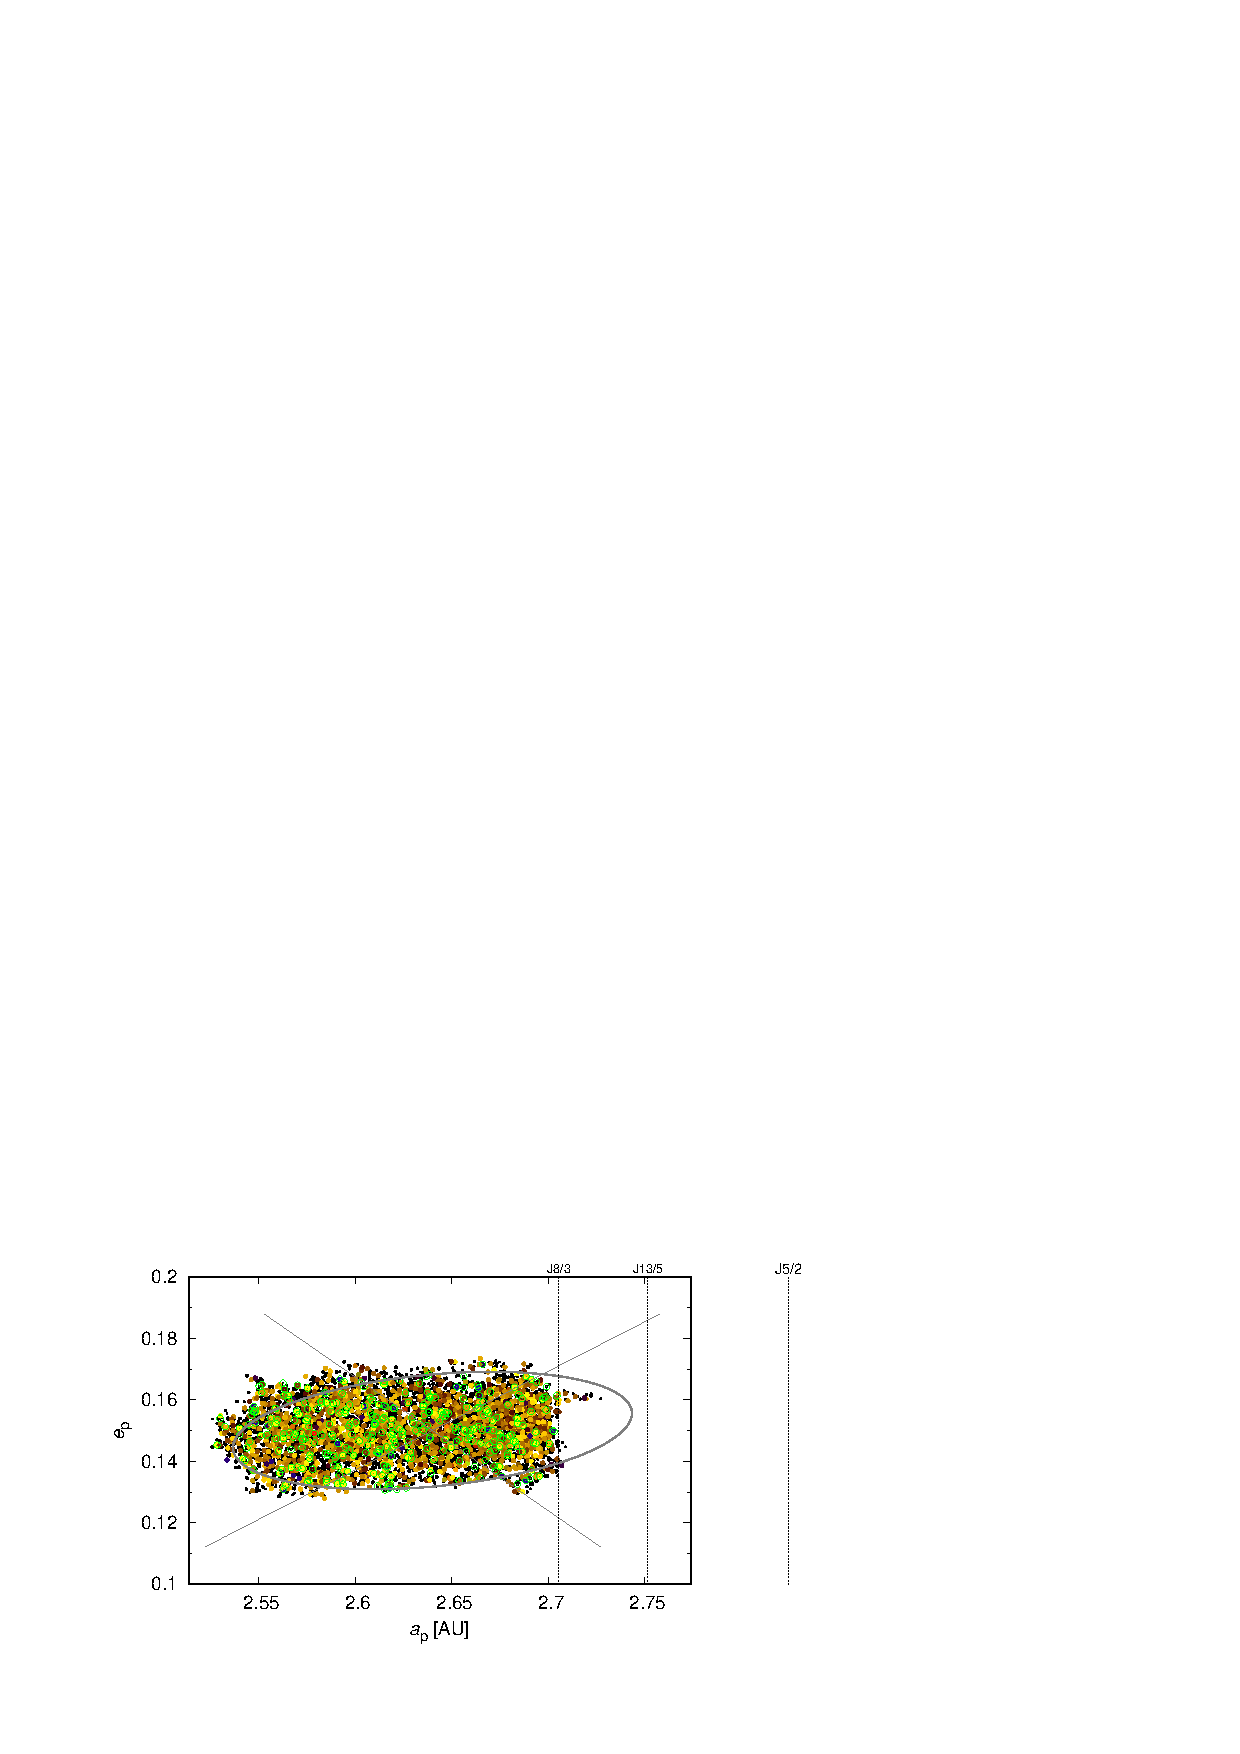
\includegraphics[width=0.5\textwidth]{obr/ae_wise}
	\caption{TODO}
	\label{ae_wise}
\end{figure}
\begin{figure}
	\centering
	\includegraphics[width=0.5\textwidth]{obr/ai_wise}
	\caption{TODO}
	\label{ai_wise}
\end{figure}
\begin{figure}
	\centering
	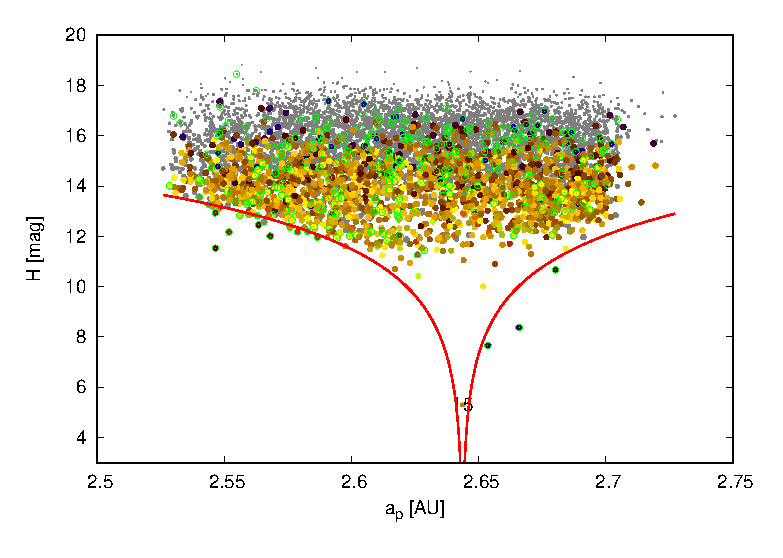
\includegraphics[width=0.5\textwidth]{obr/aH_wise}
	\caption{TODO}
	\label{aH_wise}
\end{figure}
\begin{figure}
	\centering
	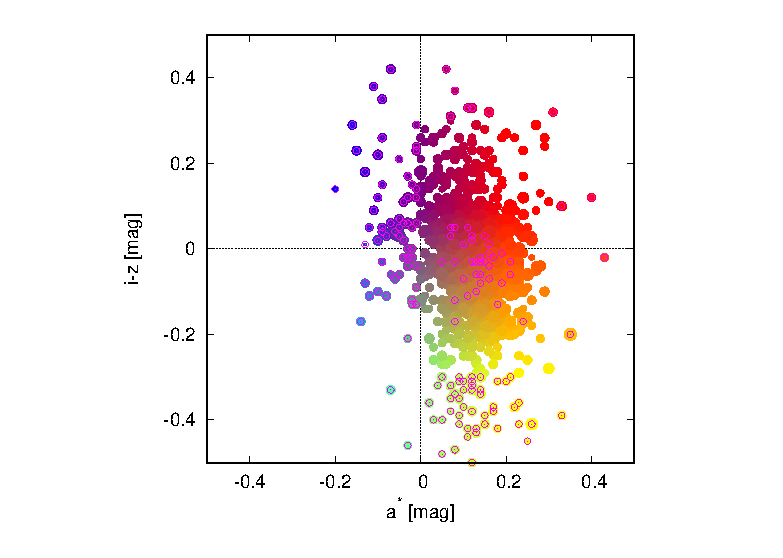
\includegraphics[width=0.5\textwidth]{obr/astar_iz}
	\caption{TODO}
	\label{astar_iz}
\end{figure}
\begin{figure}
	\centering
	\includegraphics[width=0.5\textwidth]{obr/pV_pIR}
	\caption{TODO}
	\label{pV_pIR}
\end{figure}
\begin{figure}
	\centering
	\includegraphics[width=0.5\textwidth]{obr/Nv}
	\caption{TODO}
	\label{Nv}
\end{figure}
\begin{figure}
	\centering
	\begin{subfigure}[b]{0.45\textwidth}
	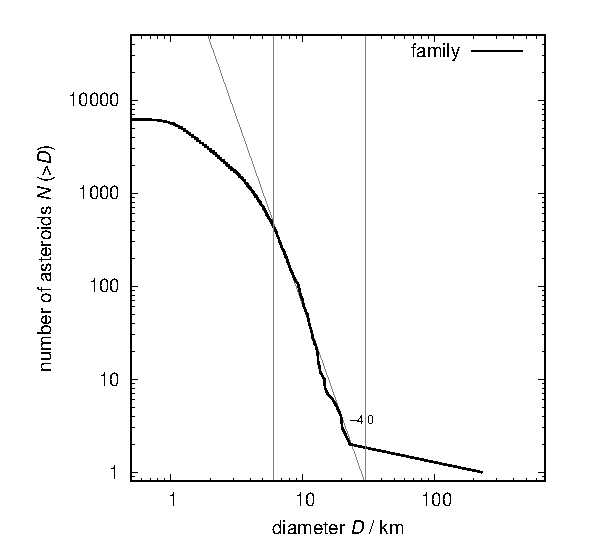
\includegraphics[width=\textwidth]{obr/size_distribution}
	\end{subfigure}
	\begin{subfigure}[b]{0.45\textwidth}
	\includegraphics[width=\textwidth]{obr/size_distribution_SMALLD}
	\end{subfigure}
	\caption{TODO}
	\label{size_distribution}
\end{figure}
\section{Nejistoty pozorovaných dat}
\section{Fyzikální model pro rodinu Eunomia}
\subsection{Jarkovského jev}
\subsection{YORP jev}
\subsection{Náhodné srážky}
\subsection{Nevratné děje při vývoji}
\section{Simulace orbitálního vývoje}
\section{Porovnání modelu a pozorování}

\chapter{Aplikace v praxi}
\chapter{Budoucí možnosti výzkumu}
\printbibliography
\end{document}
